%%%%%%%%%%%%%%%%%%%%%%%%%%%%%%%%%%%%%%%%%
% Beamer Presentation
% LaTeX Template
% Version 1.0 (10/11/12)
%
% This template has been downloaded from:
% http://www.LaTeXTemplates.com
%
% License:
% CC BY-NC-SA 3.0 (http://creativecommons.org/licenses/by-nc-sa/3.0/)
%
%%%%%%%%%%%%%%%%%%%%%%%%%%%%%%%%%%%%%%%%%

%----------------------------------------------------------------------------------------
%   PACKAGES AND THEMES
%----------------------------------------------------------------------------------------

\documentclass{beamer}

\mode<presentation> {

% The Beamer class comes with a number of default slide themes
% which change the colors and layouts of slides. Below this is a list
% of all the themes, uncomment each in turn to see what they look like.

%\usetheme{default}
%\usetheme{AnnArbor}
%\usetheme{Antibes}
%\usetheme{Bergen}
%\usetheme{Berkeley}
%\usetheme{Berlin}
%\usetheme{Boadilla}
%\usetheme{CambridgeUS}
%\usetheme{Copenhagen}
%\usetheme{Darmstadt}
%\usetheme{Dresden}
%\usetheme{Frankfurt}
%\usetheme{Goettingen}
%\usetheme{Hannover}
%\usetheme{Ilmenau}
%\usetheme{JuanLesPins}
%\usetheme{Luebeck}
\usetheme{Madrid}
%\usetheme{Malmoe}
%\usetheme{Marburg}
%\usetheme{Montpellier}
%\usetheme{PaloAlto}
%\usetheme{Pittsburgh}
%\usetheme{Rochester}
%\usetheme{Singapore}
%\usetheme{Szeged}
%\usetheme{Warsaw}

% As well as themes, the Beamer class has a number of color themes
% for any slide theme. Uncomment each of these in turn to see how it
% changes the colors of your current slide theme.

%\usecolortheme{albatross}
%\usecolortheme{beaver}
%\usecolortheme{beetle}
%\usecolortheme{crane}
%\usecolortheme{dolphin}
%\usecolortheme{dove}
%\usecolortheme{fly}
%\usecolortheme{lily}
%\usecolortheme{orchid}
%\usecolortheme{rose}
%\usecolortheme{seagull}
%\usecolortheme{seahorse}
%\usecolortheme{whale}
%\usecolortheme{wolverine}

%\setbeamertemplate{footline} % To remove the footer line in all slides uncomment this line
%\setbeamertemplate{footline}[page number] % To replace the footer line in all slides with a simple slide count uncomment this line

%\setbeamertemplate{navigation symbols}{} % To remove the navigation symbols from the bottom of all slides uncomment this line
}

\usepackage{graphicx} % Allows including images
\usepackage[utf8]{inputenc}
\usepackage[russian]{babel}
\usepackage{booktabs} % Allows the use of \toprule, \midrule and \bottomrule in tables
\usepackage{adjustbox}

%----------------------------------------------------------------------------------------
%   TITLE PAGE
%----------------------------------------------------------------------------------------

\title[SDSJ]{Обзор данных конкурса от ``Сбербанк''} % The short title appears at the bottom of every slide, the full title is only on the title page

\author{Оспанов Аят} % Your name
\institute[] % Your institution as it will appear on the bottom of every slide, may be shorthand to save space
{
517 группа \\ % Your institution for the title page
}
\date{} % Date, can be changed to a custom date

\begin{document}

\begin{frame}
\titlepage % Print the title page as the first slide
\center{Москва, 2016}
\end{frame}

% \begin{frame}
% \frametitle{Overview} % Table of contents slide, comment this block out to remove it
% \tableofcontents % Throughout your presentation, if you choose to use \section{} and \subsection{} commands, these will automatically be printed on this slide as an overview of your presentation
% \end{frame}

%----------------------------------------------------------------------------------------
%   PRESENTATION SLIDES
%----------------------------------------------------------------------------------------

%------------------------------------------------
\section{First Section} % Sections can be created in order to organize your presentation into discrete blocks, all sections and subsections are automatically printed in the table of contents as an overview of the talk
%------------------------------------------------

% \subsection{Subsection Example} % A subsection can be created just before a set of slides with a common theme to further break down your presentation into chunks

\begin{frame}
\frametitle{Какой день недели?}

\begin{figure}
    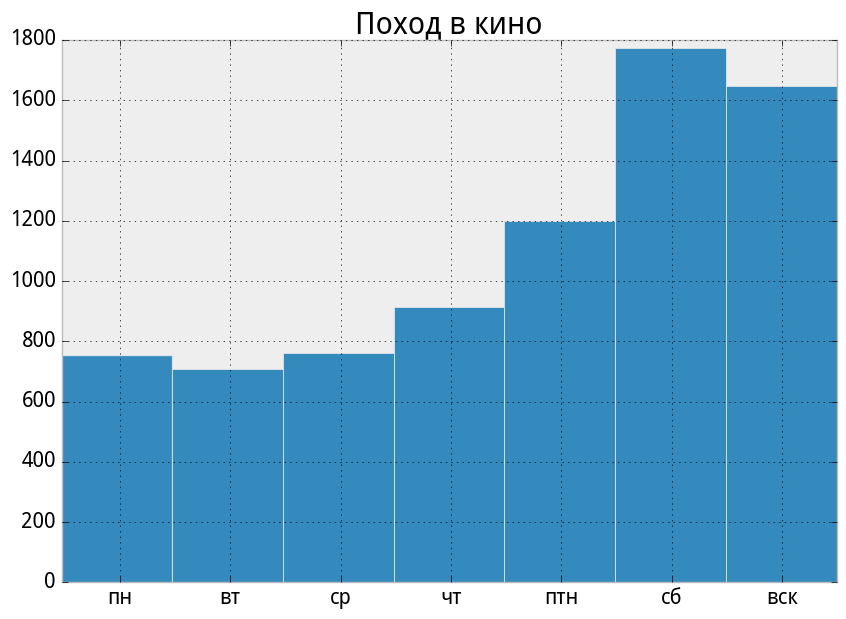
\includegraphics[height=0.5\linewidth]{pics/day_of_week.png}
\end{figure}

\center{Смещение на 4 дня}

\end{frame}

%------------------------------------------------

\begin{frame}
\frametitle{Транзакции по дням}

\begin{figure}
    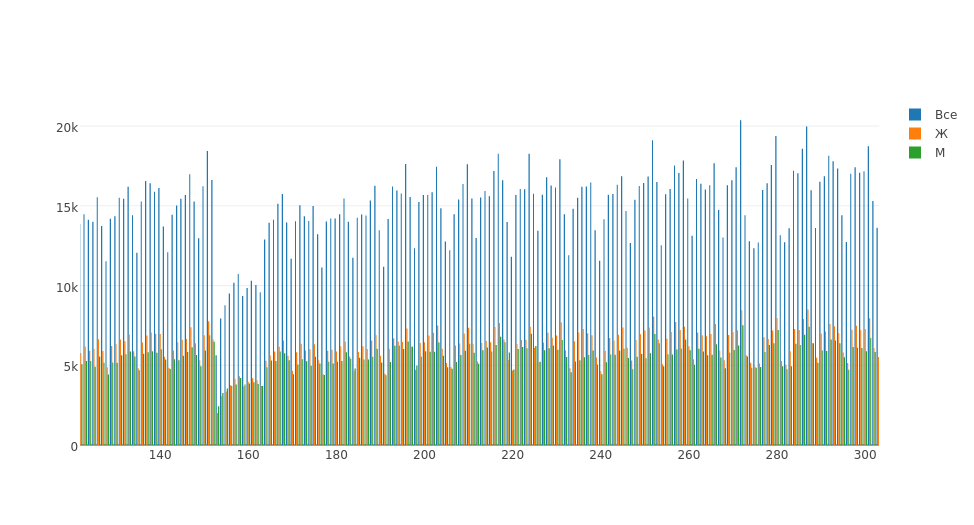
\includegraphics[width=1\linewidth]{pics/trans_all.png}
\end{figure}

\center{Какой год?}

\end{frame}

%------------------------------------------------

\begin{frame}
\frametitle{Какой год?}

Точно знаем:
\begin{itemize}
    \item 153 день - 1 января, четверг
    \item 272 день - 31 апреля, далее 4 дня выходных на майские праздники
\end{itemize}

Предположения:
\begin{itemize}
    \item 206 день, пнд - 23 февраля
    \item 219 день, вск - 8 марта
\end{itemize}

\end{frame}

%------------------------------------------------

\begin{frame}
\frametitle{219 день - 8 марта}

\begin{figure}
    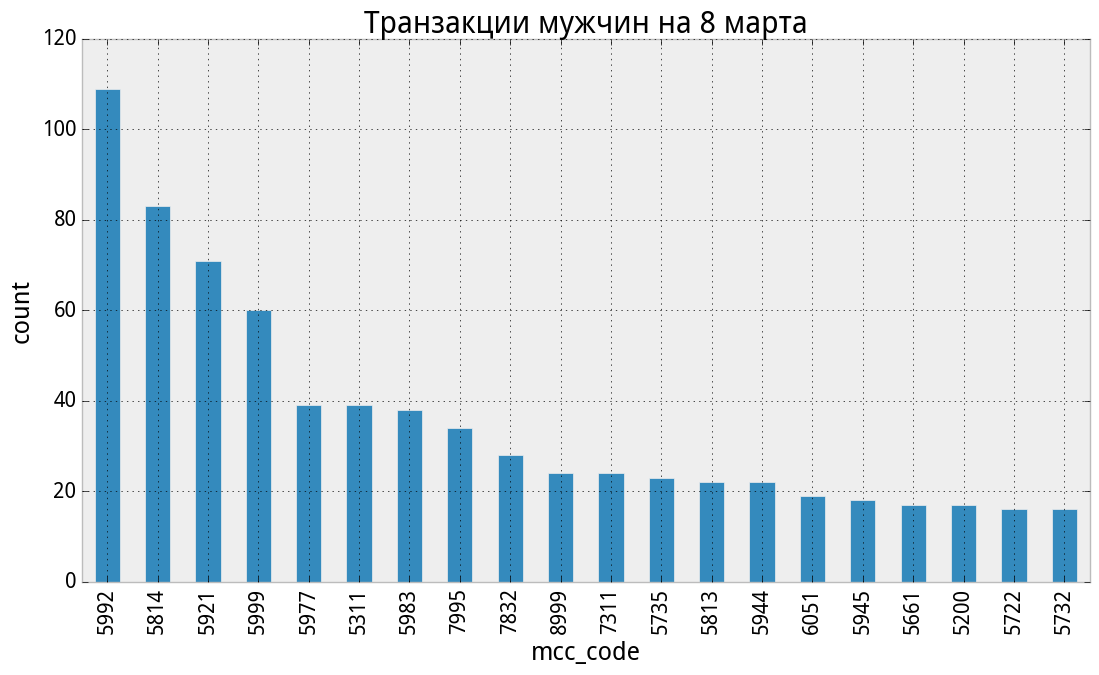
\includegraphics[width=1\linewidth]{pics/men_8mar.png}
\end{figure}

\end{frame}

%------------------------------------------------

\begin{frame}
\frametitle{219 день - 8 марта}

\begin{adjustbox}{width=1\textwidth}
\begin{tabular}{lll}
    mcc\_code & amount & mcc\_description                                                    \\
    5992      & 109    & Флористика                                                          \\
    5814      & 83     & Рестораны, закусочные                                               \\
    5921      & 71     & Магазины с продажей спиртных напитков на вынос (пиво, вино и ликер) \\
    5999      & 60     & Плавательные бассейны — распродажа                                  \\
    5977      & 39     & Магазины косметики                                                  \\
    5311      & 39     & Универмаги                                                          \\
    5983      & 38     & Горючее топливо — уголь, нефть, разжиженный бензин, дрова           \\
    7995      & 34     & Транзакции по азартным играм                                        \\
    7832      & 28     & Кинотеатры                                                          \\
    8999      & 24     & Профессиональные услуги, нигде ранее не классифицируемые            \\
    7311      & 24     & Рекламные услуги                                                    \\
    5735      & 23     & Магазины звукозаписи                                                \\
    5813      & 22     & Бары, коктейль-бары, дискотеки, ночные клубы и таверны ...          \\
    5944      & 22     & Магазины по продаже часов, ювелирных изделий и изделий из серебра   \\
    6051      & 19     & Не-финансовые институты — иностранная валюта, денежные переводы ... \\
    5945      & 18     & Магазины игрушек                                                    \\
    5661      & 17     & Обувные магазины                                                    \\
    5200      & 17     & Товары для дома                                                     \\
    5722      & 16     & Бытовое оборудование                                                \\
    5732      & 16     & Продажа электронного оборудования
\end{tabular}
\end{adjustbox}

\end{frame}

%------------------------------------------------

\begin{frame}
\frametitle{219 день - 8 марта}

\begin{figure}
    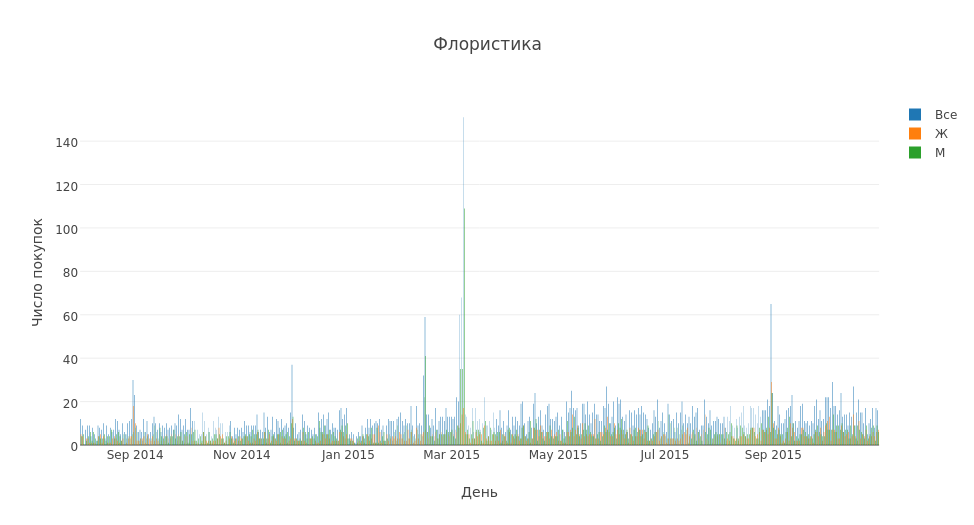
\includegraphics[width=1\linewidth]{pics/flowers_8mar.png}
\end{figure}

\end{frame}

%------------------------------------------------

\begin{frame}
\frametitle{219 день - 8 марта}

\begin{figure}
    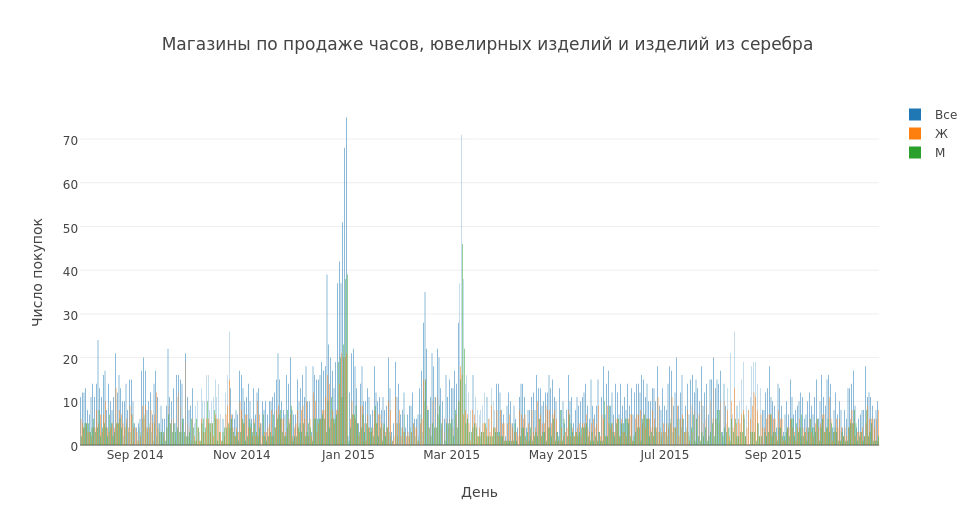
\includegraphics[width=1\linewidth]{pics/jewel_8mar.png}
\end{figure}

\end{frame}

%------------------------------------------------

\begin{frame}
\frametitle{206 день - 23 февраля}

\begin{figure}
    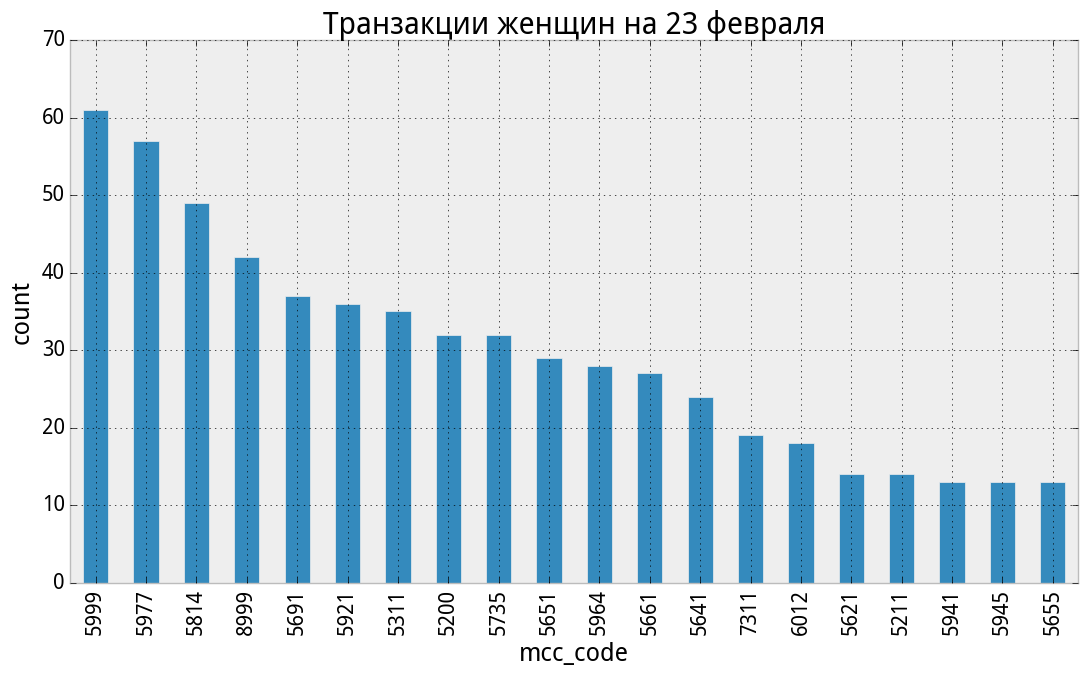
\includegraphics[width=1\linewidth]{pics/women_23feb.png}
\end{figure}

\end{frame}

%------------------------------------------------

\begin{frame}
\frametitle{206 день - 23 февраля}

\begin{adjustbox}{width=1\textwidth}
\begin{tabular}{lll}
    mcc\_code & amount & mcc\_description                                                    \\
    5999      & 61     & Плавательные бассейны — распродажа                                  \\
    5977      & 57     & Магазины косметики                                                  \\
    5814      & 49     & Рестораны, закусочные                                               \\
    8999      & 42     & Профессиональные услуги, нигде ранее не классифицируемые            \\
    5691      & 37     & Магазины мужской и женской одежды                                   \\
    5921      & 36     & Магазины с продажей спиртных напитков на вынос (пиво, вино и ликер) \\
    5311      & 35     & Универмаги                                                          \\
    5200      & 32     & Товары для дома                                                     \\
    5735      & 32     & Магазины звукозаписи                                                \\
    5651      & 29     & Одежда для всей семьи                                               \\
    5964      & 28     & Прямой маркетинг — торговля через каталог                           \\
    5661      & 27     & Обувные магазины                                                    \\
    5641      & 24     & Детская одежда, включая одежду для самых маленьких                  \\
    7311      & 19     & Рекламные услуги                                                    \\
    6012      & 18     & Финансовые институты — торговля и услуги                            \\
    5621      & 14     & Готовая женская одежда                                              \\
    5211      & 14     & Лесо- и строительный материал                                       \\
    5941      & 13     & Магазины спорттоваров                                               \\
    5945      & 13     & Магазины игрушек                                                    \\
    5655      & 13     & Спортивная одежда, одежда для верховой езды и езды на мотоцикле
\end{tabular}
\end{adjustbox}

\end{frame}

%------------------------------------------------

\begin{frame}
\frametitle{206 день - 23 февраля}

\begin{figure}
    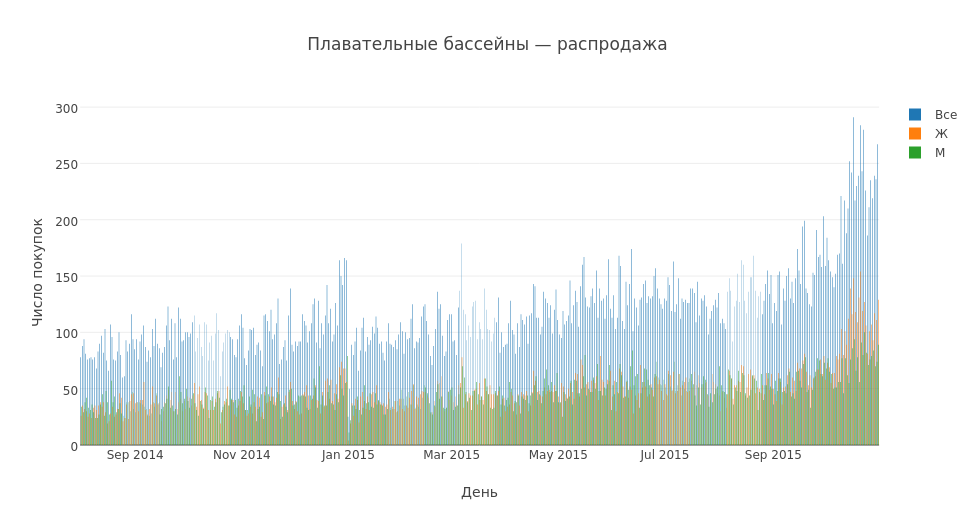
\includegraphics[width=1\linewidth]{pics/swim_23feb.png}
\end{figure}

\end{frame}

%------------------------------------------------

\begin{frame}
\frametitle{Затраты по дням}

\begin{figure}
    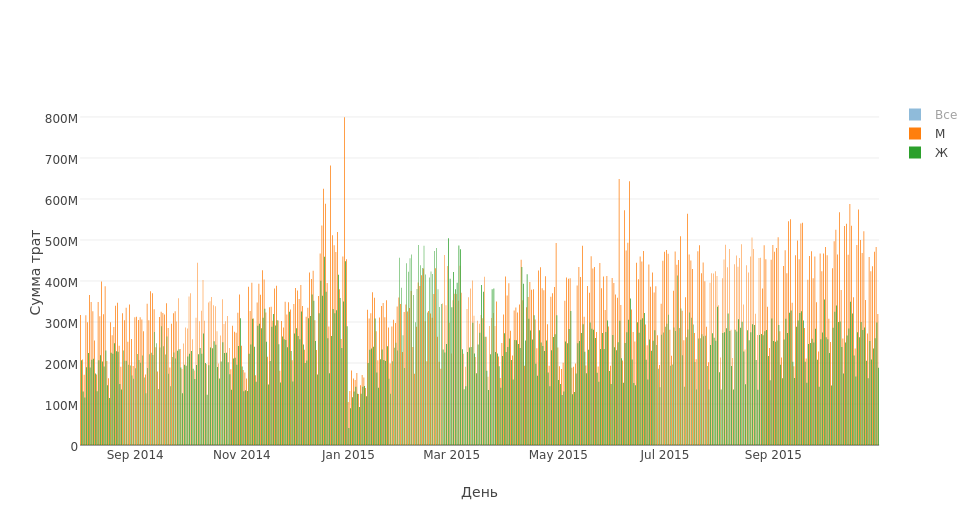
\includegraphics[width=1\linewidth]{pics/minus.png}
\end{figure}

\end{frame}

%------------------------------------------------

\begin{frame}
\frametitle{Доходы по дням}

\begin{figure}
    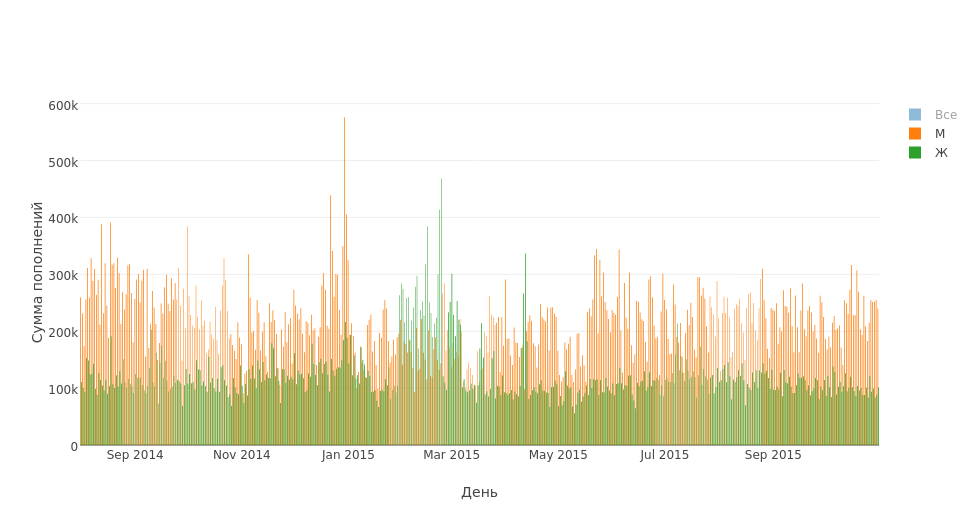
\includegraphics[width=1\linewidth]{pics/plus.png}
\end{figure}

\end{frame}

%------------------------------------------------

\begin{frame}
\frametitle{Восстаноление суммы}

Рассмотрим суммы, снятых с карточек. Банкомат не выдает такие суммы

\begin{figure}
    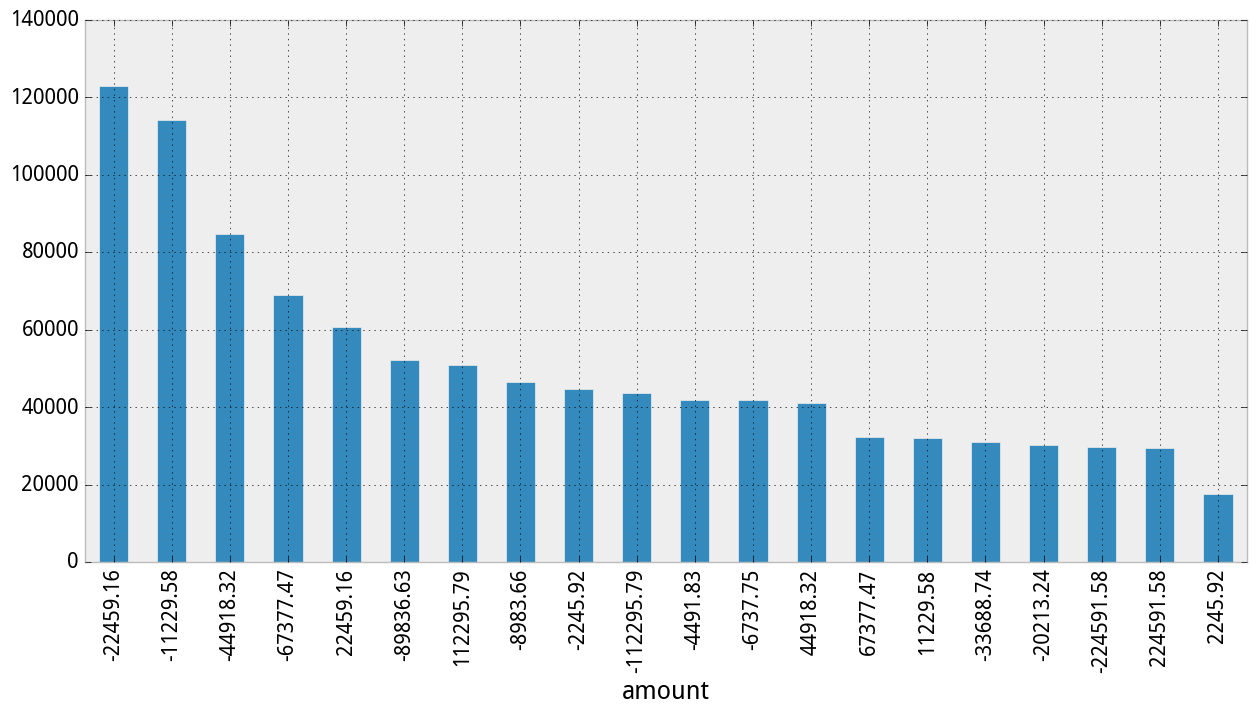
\includegraphics[width=1\linewidth]{pics/amount_count.png}
\end{figure}

\end{frame}

%------------------------------------------------

\begin{frame}
\frametitle{Восстаноление суммы}

Предположим, что преобразование линейное. Тогда $sum_{original} = 0.044525267266723685 * sum_{converted}$

\begin{figure}
    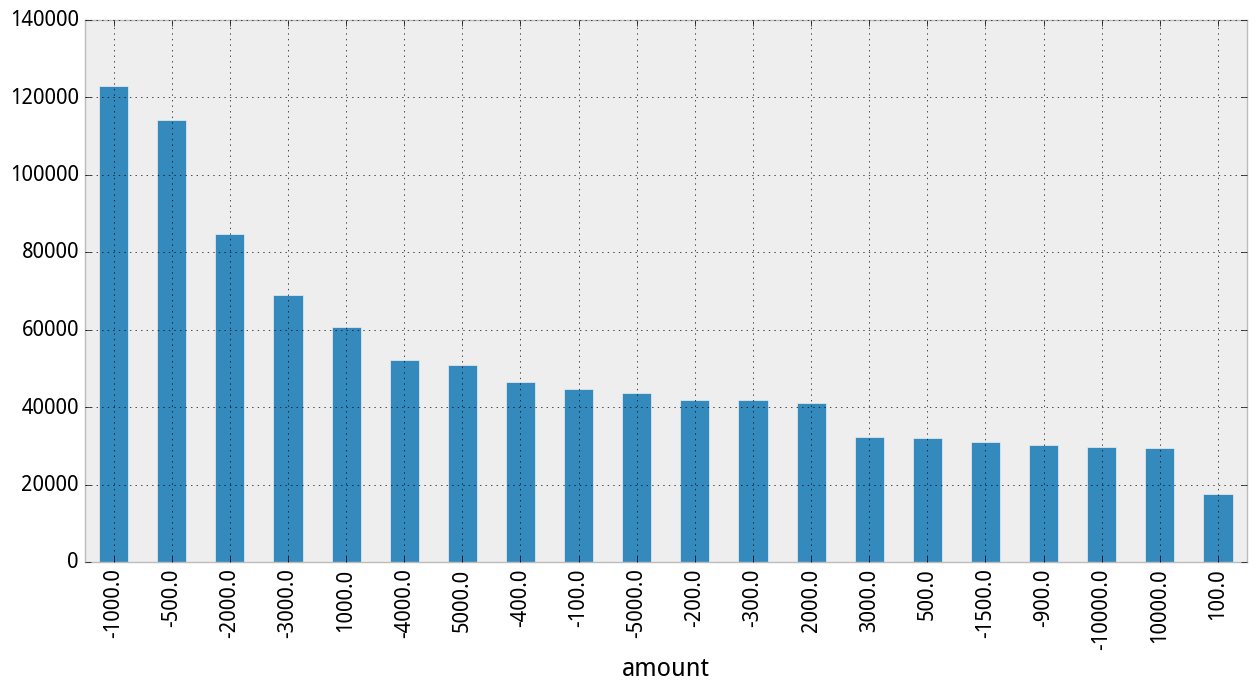
\includegraphics[width=1\linewidth]{pics/amount_count_conv.png}
\end{figure}

Предположение верно!

\end{frame}

%------------------------------------------------

\begin{frame}
\frametitle{Выводы}

\begin{itemize}
    \item Мужчины дарят цветы в основном только на 8 марта =)
    \item Женщины получают украшения еще и на новый год
    \item Женщины тратят на 23 февраля больше, чем в среднем за год, но при этом умудряются не тратиться
    \item Преобразование сумм не такое уж и трудное
    \item Не удалось найти себя =(
\end{itemize}

\end{frame}

%------------------------------------------------

\begin{frame}
\LARGE{\centerline{Спасибо за внимание!}}
\end{frame}

%----------------------------------------------------------------------------------------

\end{document}